\documentclass{scrartcl}
\usepackage{parskip}
\usepackage[utf8]{inputenc}
\usepackage[T1]{fontenc}
\usepackage[ngerman]{babel}
\usepackage{amsmath}
\usepackage{listings}
\usepackage{graphicx}

\lstset{basicstyle=\ttfamily,columns=fixed}

\begin{document}

\section{Spieleprogrammierung mit GIF-Streams}

Snake ist ein Computerspiel, bei dem man eine Schlange duch ein Spielfeld steuert.
Futter zu essen verlängert die Schlange.
Prallt die Schlange an eine Wand oder sich selbst, so endet das Spiel.

\begin{center}

\includegraphics{snake}
\end{center}

In dieser Aufgabe implementieren Sie Snake in Haskell.
Das dazu benötigte Rahmenwerk finden Sie auf der Übungshomepage.

Die Ausgabe des Spiels soll ein GIF-Stream sein, den man im Browser anschauen kann, um so das Spiel live mitzuverfolgen.
Es werden 64 Farben unterstützt, die als Int-Tupel von (0,0,0) bis (3,3,3) angesprochen werden.

\begin{lstlisting}
type RGB = (Int,Int,Int)
\end{lstlisting}

Ein einzelner Frame einer GIF ist definiert als Liste von Zeilen, wobei jede Zeile eine Liste von RGB-Werten ist.

\begin{lstlisting}
type Frame = [[RGB]]
\end{lstlisting}

Das Rahmenwerk stellt eine Funktion \texttt{server} zur Verfügung, die einen HTTP-Server unter dem angegebenen Port startet.
Der Server schickt jedem Client in einem festgelegten Intervall einen neuen Frame der GIF-Animation.
In der übergebenen Logic-Funktion werden dynamisch neue Frames generiert.

\begin{lstlisting}
server :: PortNumber -> Int -> Logic -> IO ()
\end{lstlisting}

Die Datei \texttt{Snake.hs} enthält das Grundgerüst für das zu schreibende Snake-Spiel.
Kompilieren Sie das Spiel und führen Sie es aus:

\begin{lstlisting}
$ ghc Snake.hs
[1 of 2] Compiling GifStream        ( GifStream.hs, GifStream.o )
[2 of 2] Compiling Main             ( Snake.hs, Snake.o )
Linking Snake ...
$ ./Snake
Listening on http://127.0.0.1:5002/
\end{lstlisting}

Öffnen Sie die angegebene Adresse in Ihrem Browser.
Durch drücken der Tasten WASD im Terminal lässt sich die Ausgabe im Browser beeinflussen.

Anderen Teilnehmern Ihres Netzwerks ist es ebenfalls möglich den GIF-Stream zu betrachten, indem Sie statt \texttt{127.0.0.1} Ihre Netzwerk-IP-Adresse eintragen.

Desweiteren ist es möglich den GIF-Stream aufzunehmen um ihn später anzuschauen:

\begin{lstlisting}
wget -O game.gif http://127.0.0.1:5002/
\end{lstlisting}

Die wichtigste Funktion in \texttt{Snake.hs} ist \texttt{logic}:

\begin{lstlisting}
logic wait getInput frameSignal = initialState >>= go
  where
    go (State oldAction snake food) = do
      input <- getInput

      -- Generate new state
      let action = charToAction input oldAction
      let newSnake = snake
      let newFood = food

      let frame = case action of
            MoveUp    -> replicate height $ replicate width (3,0,0)
            MoveDown  -> replicate height $ replicate width (0,3,0)
            MoveLeft  -> replicate height $ replicate width (0,0,3)
            MoveRight -> replicate height $ replicate width (3,3,3)

      sendMSignal frameSignal $ scale zoom frame

      wait
      go $ State action newSnake newFood
\end{lstlisting}

Die Funktion \texttt{logic} erzeugt einen initialen Zustand für das Snake-Spiel und übergibt diesen an die \texttt{go}-Funktion.
Diese liest mit \texttt{getInput} die zuletzt gedrückte Taste.
Anschließend wird ein neuer Spielzustand generiert.
Der anzuzeigende Frame wird dabei abhängig von der gedrückten Taste gewählt.
Schließlich wird mit \texttt{sendMSignal} ein neuer Frame an alle verbundenen Clients geschickt.
Dabei wird jeder Frame durch \texttt{scale} vergrößert.
Der Aufruf von \texttt{wait} bewirkt ein Warten für die vereinbarte Zeit \texttt{delay}, die standardmäßig auf $200 ms$ gesetzt ist.
Am Ende der Funktion ruft diese sich selbst endrekursiv mit dem neu generierten Zustand auf.

Ziel dieser Aufgabe ist es die Spiellogik in der Funktion \texttt{logic} schrittweise zu erweitern, so dass man am Ende Snake spielen kann.

\subsection{Spielfeld ausgeben}
Erzeugen Sie aus dem aktuellen Zustand ein Bild und geben Sie dieses aus statt der einfachen farbigen Bilder.

Schreiben Sie dazu eine Liste \texttt{imgPositions}, die die Koordinaten des Spielfelds an ihrer jeweiligen Position speichert.

\begin{lstlisting}
imgPositions :: [[Position]]
\end{lstlisting}

Die Größe des Feldes ist dabei in \texttt{width} und \texttt{height} gespeichert.
Für ein Feld der Größe 3x4 würde imgPositions wie folgt aussehen:

\begin{lstlisting}
imgPositions = [[(0,0),(1,0),(2,0)]
               ,[(0,1),(1,1),(2,1)]
               ,[(0,2),(1,2),(2,2)]
               ,[(0,3),(1,3),(2,3)]]
\end{lstlisting}

Implementieren Sie eine Funktion \texttt{colorize}, die eine einzelne Bildposition auf eine Farbe abbildet, so dass sich der neue Frame durch \texttt{let frame = map (map (colorize newSnake newFood)) imgPositions} erzeugen lässt.
Ein Feld soll verschieden eingefärbt werden, je nachdem ob diese Position Teil der Schlange, Futterstück, oder Hintergrund ist.

\begin{lstlisting}
colorize :: [Position] -> Position -> Position -> RGB
\end{lstlisting}

\subsection{Verhalten Schlange}
Implementieren Sie nun die Zustandsänderung der Schlange, so dass Sie in der Spiellogik \texttt{let newSnake = moveSnake snake food action} schreiben können.

\begin{lstlisting}
moveSnake :: [Position] -> Position -> Action -> Position
\end{lstlisting}

Eine Schlange ist als Liste von Positionen definiert.
Die neue Schlange erhält abhängig von der übergebenen Aktion einen neuen Kopf.
Beim Schwanz wird das letzte Element abgeschnitten, außer wenn die Schlange gerade auf Futter gestoßen ist.

Es muss sichergestellt werden, dass die vom Benutzer gewählte Aktion überhaupt möglich ist.
Schreiben Sie dazu eine Funktion \texttt{validateAction}, so dass sie in der Spiellogik \texttt{let action = validateAction oldAction \$ charToAction input oldAction} schreiben können.
Dazu soll \texttt{validateAction} nur dann eine neue Aktion zurückgeben, wenn diese möglich ist.
Ansonsten soll die alte Aktion zurückgegeben werden.

%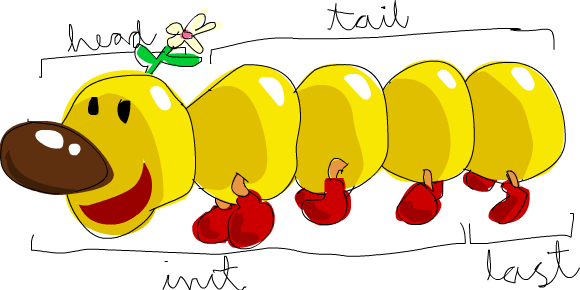
\includegraphics[width=\textwidth]{listmonster}

\subsection{Verhalten Futter}
Implementieren Sie nun die Zustandsänderung des Futters, so dass Sie in der Spiellogik \texttt{newFood <- moveFood newSnake food} schreiben können.

\begin{lstlisting}
moveFood :: [Position] -> Position -> IO Position
\end{lstlisting}

Wenn die Schlange gerade das Futter nicht isst, kann direkt die alte Position des Futters zurückgegeben werden.
Ansonsten soll die neue Position des Futters zufällig gewählt werden.
Vermeiden Sie dass das Futter im Körper der Schlange erscheint.

Zufallszahlen zwischen $x$ und $y$ (einschließlich) lassen sich bei Verwendung der do-Syntax mit \texttt{r <- randomRIO (x,y)} generieren.
Importieren Sie dazu \texttt{System.Random}.

\subsection{Spielende}
Passen Sie das Ende von \texttt{logic} so an, dass mit \texttt{checkGameOver newSnake} die Gültigkeit des neuen Zustands überprüft wird.
Bei einem ungültigen Zustand soll das Spiel durch Aufruf von \texttt{initialState >>= go} neugestartet werden.

\begin{lstlisting}
checkGameOver :: [Position] -> Bool
\end{lstlisting}

\subsection{Kür}
Schreiben Sie ein weiteres Spiel mit GIF-Stream-Ausgabe, zum Beispiel Pong, Tetris oder Conway's Game of Life.
\end{document}
